\section{Deep Learning}

In the field of machine learning, the first models you
are often introduced to are those for regression
and classification that utilize linear
combinations of fixed basis functions.
According to \cite{Bishop:2008aa},
these models possess useful analytical and computational properties,
but their practical applicability is constrained 
since their capacity is limited to linear functions
and they cannot understand the interaction between any two input variables.
This leads to problems such as the curse of dimensionality,
where the number of possible interactions between variables grows exponentially
with the number of input variables.
To address large-scale problems, it is essential to adapt the basis functions
to the data, as demonstrated by support vector machines (SVMs).
Alternatively, one can fix the number of basis functions in advance while
allowing them to be adaptive, utilizing parametric forms for the basis
functions with parameter values adjusted during training.

The most successful example of this approach in pattern recognition is the
\textbf{feed-forward neural network},
also known as the multilayer perceptron (MLP).
\begin{figure}[h]
    \centering
    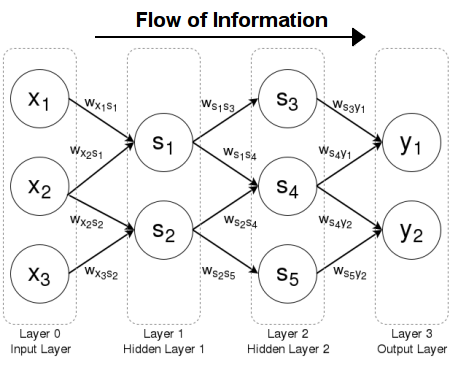
\includegraphics[width=.9\textwidth]{figures/ch3/1.mlp.png}
    \caption{A feed-forward neural network with two hidden layers}
    \vspace{-10px}
    \caption*{\scriptsize{Source: \href{https://brilliant.org/wiki/feedforward-neural-networks/}{Brilliant}}}
    \label{fig:mlp}
\end{figure}

As explained in 
\cite{goodfellow2016deep},
the goal of a feedforward network is to approximate a specific function
\( f^* \). For example, in a classification task,
\( y = f^*(x) \) maps an input \( x \) to a category \( y \).
A feedforward network defines a mapping \( y = f(x; \theta) \) and
learns the parameters \( \theta \) that yield the best approximation
of this function.

These models are called \textbf{feedforward} because information
flows unidirectionally from the input \( x \), through intermediate computations
defining \( f \), and ultimately to the output \( y \), without feedback loops.

The training data directly specifies the output layer's behavior but
not the intermediate layers, which are called \textbf{hidden layers}
because their desired outputs are not provided by the training data.
The learning algorithm must determine how to best utilize these
hidden layers to approximate \( f^* \).
Every layer of the network computes a non-linear transformation of the
previous layer's activations, this way a complex function can be
approximated by composing simpler functions, one for each layer.
Layers are composed of a set of units, where each unit is a node that
computes a non-linear function of the weighted sum of its inputs
and is only connected to units in the previous and the following layer.

A feedforward network is called a \textbf{deep neural network} if it has
more than one hidden layer, the branch of machine learning that studies
deep neural networks is called \textbf{deep learning}.

They are called networks due to their structure, which involves composing
multiple functions together. Typically, this composition is represented
by a directed acyclic graph. For instance, functions
\( f^{(1)} \), \( f^{(2)} \), and \( f^{(3)} \) might be connected in
a chain to form \( f(x) = f^{(3)}(f^{(2)}(f^{(1)}(x))) \).

Functions \( f^{(1)} \) and \( f^{(2)} \) must
be non linear, otherwise the composition would collapse into a single
linear function. These non-linear functions are
called \textbf{activation functions}.
The last function \( f^{(3)} \) is typically a linear function that maps
the output of the final hidden layer to the output layer.
This is the same as applying a linear model to a transformed
input \( \phi(x) \), where \( \phi \) is a nonlinear transformation.
The question then becomes how to choose the mapping \( \phi \).

The strategy of deep learning is to learn \( \phi \):
in this approach, we use a model
\[ y = f(x; \theta, w) = \phi(x; \theta)^\top w \]
Here, we have parameters \( \theta \) that are used to learn \( \phi \)
from a broad class of functions, and parameters \( w \) that map \( \phi(x) \)
to the desired output.
This approach allows for greater flexibility:
specifically, by using a broad family of functions
\( \phi(x; \theta) \), the human designer only needs to select the appropriate
general function family rather than finding precisely an exact function.

The \textbf{universal approximation theorem} \cite{HORNIK1989359}
tells us that regardless of what function
we are trying to learn, we know that a feedforward network with enough units
will be able to \emph{represent} this
function, however we are not guaranteed that the training algorithm will be able
to \emph{learn} it.

\section{Reinformcement Learning}

``\textbf{Reinforcement learning} is learning [...] how
to map situations to actions so
as to maximize a numerical reward signal.
The learner is not told which actions to
take, but instead must discover which actions
yield the most reward by trying them. In
the most interesting and challenging cases, actions may
affect not only the immediate
reward but also the next situation and,
through that, all subsequent rewards.
These two
characteristics, \textbf{trial-and-error search} and \textbf{delayed reward},
are the two most important
distinguishing features of reinforcement learning.'' \cite{sutton1998}

Let's explore the basic concepts of reinforcement learning with
a simple example as described in \cite{zhao2024RLBook}.
Consider a grid world scenario as shown in Figure \ref{fig:rl}
where a robot, referred to as
the \textbf{agent}, moves between cells, occupying one cell at a time.
The white cells are accessible, while the orange cells are forbidden.
The goal is for the agent to reach a target cell.

\begin{figure}[h]
    \centering
    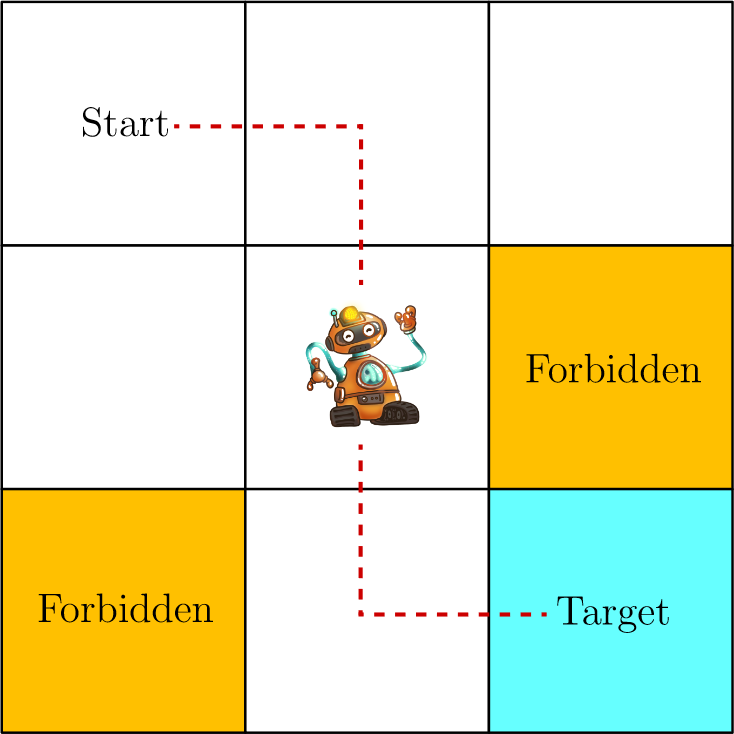
\includegraphics[width=.5\textwidth]{figures/ch3/2.rl.png}
    \caption{A simple reinforcement learning task}
    \vspace{-10px}
    \caption*{\scriptsize{Source: \cite{zhao2024RLBook}}}
    \label{fig:rl}
\end{figure}

To achieve this, the agent needs a \textbf{policy} that guides it to the target
efficiently, avoiding forbidden cells and unnecessary detours.
If the grid layout is known, planning is simple.
However, without prior knowledge, the agent must explore and learn
through trial and error.

The agent's status in the grid is defined by its \textbf{state}
\( s_i \in \mathcal{S} \), which represents its location relative
to the \textbf{environment}.
In the examples with nine cells, the state space is
\( \mathcal{S} = \{s_1, s_2, \ldots, s_9\} \)..

From each state, the agent can perform five \textbf{actions}: move up,
right, down, left or stay put, denoted as \( a_1, a_2, \ldots, a_5 \),
this set of actions is the action space
\( \mathcal{A} = \{a_1, \ldots, a_5\} \).
The available actions can vary by state, for instance,
at \( s_1 \), actions \( a_1 \) (up) and \( a_4 \) (left) would collide
with the grid boundary, so the action space is
\( \mathcal{A}(s_1) = \{a_2, a_3, a_5\} \).

When taking an action, the agent may move from one state to another,
a process known as \textbf{state transition}. For example,
if the agent is at state \( s_1 \) and selects action
\( a_2 \) (moving rightward), it transitions to state
\( s_2 \). This process can be represented as:
\[ s_1 \overset{a_2}{\longrightarrow} s_2 \]
The state transition process is defined for each
state and its associated actions. Mathematically, state transitions
are described by conditional probabilities.
For example, for \( s_1 \) and \( a_2 \),
the conditional probability distribution is:
\[
\begin{aligned}
p(s_1 \mid s_1, a_2) &= 0, \\
p(s_2 \mid s_1, a_2) &= 1, \\
p(s_3 \mid s_1, a_2) &= 0, \\
p(s_4 \mid s_1, a_2) &= 0, \\
p(s_5 \mid s_1, a_2) &= 0,
\end{aligned}
\]
indicating that taking \( a_2 \) at \( s_1 \) guarantees
the agent moves to \( s_2 \), with a probability of one,
and zero probability for other states.

This is a deterministic state transition,
but state transitions can also be stochastic,
requiring conditional probability distributions.
For instance, if random wind gusts affect the grid,
taking action \( a_2 \) at \( s_1 \) might blow the agent to \( s_5 \)
instead of \( s_2 \), resulting in \( p(s_5 \mid s_1, a_2) > 0 \).

A \textbf{policy} is a function that maps states to actions,
indicating the agent's behavior in the environment.
In other words, a policy tells the agent what action to take
at each state.

Mathematically, policies can be described by conditional probabilities. Denote the policy in Figure 1.4 as \( \pi(a \mid s) \), a conditional probability distribution function defined for every state. For example, the policy for \( s_1 \) is:
\[
\begin{aligned}
\pi(a_1 \mid s_1) &= 0, \\
\pi(a_2 \mid s_1) &= 1, \\
\pi(a_3 \mid s_1) &= 0, \\
\pi(a_4 \mid s_1) &= 0, \\
\pi(a_5 \mid s_1) &= 0,
\end{aligned}
\]
indicating that the probability of taking action \( a_2 \) at state \( s_1 \) is one, and the probabilities of taking other actions are zero.

The above policy is deterministic, but policies may generally be stochastic. For instance, the policy in Figure 1.5 is stochastic: at state \( s_1 \), the agent may take actions to move either rightward or downward, each with a probability of 0.5. In this case, the policy for \( s_1 \) is:
\[
\begin{aligned}
\pi(a_1 \mid s_1) &= 0, \\
\pi(a_2 \mid s_1) &= 0.5, \\
\pi(a_3 \mid s_1) &= 0.5, \\
\pi(a_4 \mid s_1) &= 0, \\
\pi(a_5 \mid s_1) &= 0.
\end{aligned}
\]

After executing an action at a state, the agent receives a
reward \( r \) as feedback from the environment.
The \textbf{reward} is a function of the state \( s \) and action \( a \),
denoted as \( r(s, a) \) and it can be positive, negative, or zero.
Different rewards influence the policy the agent learns.
Generally, a positive reward encourages the agent to take the
corresponding action, while a negative reward discourages it.

However we can't find good policies
by simply selecting actions with the greatest immediate rewards
since they do not consider
long-term outcomes. To determine a good policy, we must consider the total
reward obtained in the long run and
an action with the highest immediate reward may not lead to
the greatest total reward.

A \textbf{trajectory} is a state-action-reward chain.
For example, the agent in our example may follow this trajectory:
\[ s_1 \xrightarrow{a_2, r=0} s_2 \xrightarrow{a_3, r=0} s_5 \xrightarrow{a_3, r=0} s_8 \xrightarrow{a_2, r=1} s_9. \]
The return of this trajectory is the sum of all rewards collected along it:
\[\text{return} = 0+0+0+1=1\]
\textbf{Returns}, also called total rewards or cumulative rewards,
are used to evaluate policies.
Returns can also be defined for infinitely long trajectories, which may diverge.
Therefore, we introduce the concept of \textbf{discounted return} for infinitely
long trajectories. The discounted return is the sum of the discounted rewards:
\[
\text{discounted return} = 0 + \gamma \cdot 0 + \gamma^2 \cdot 0 + \gamma^3 \cdot 1 + \gamma^4 \cdot 1 + \gamma^5 \cdot 1 + \ldots,
\]
where \( \gamma \in (0, 1) \) is the discount rate.
If \( \gamma \) is close to 0, the agent emphasizes near-future rewards,
resulting in a short-sighted policy. If \( \gamma \) is close to 1,
the agent emphasizes far-future rewards.

When following a policy, the agent may stop at \textbf{terminal states},
resulting in a trajectory called an \textbf{episode}.

The framework of \textbf{Markov Decision Processes} (MDPs)
allows us to formally presents these concepts.
An MDP is a general framework for describing stochastic dynamical systems
and its key components are:
\begin{itemize}
    \item \textbf{Sets:}
    \begin{itemize}
        \item \textbf{State space:} The set of all states,
        denoted as \( \mathcal{S} \).
        \item \textbf{Action space:} The set of actions,
        denoted as \( \mathcal{A}(s) \), associated with each state
        \( s \in \mathcal{S} \).
        \item \textbf{Reward set:} The set of rewards,
        denoted as \( \mathcal{R}(s, a) \), associated with each state-action
        pair \((s, a)\).
    \end{itemize}
    \item \textbf{Model:}
    \begin{itemize}
        \item \textbf{State transition probability:} At state \( s \),
        when taking action \( a \), the probability of transitioning to state
        \( s' \) is \( p(s' \mid s, a) \).\\
        It holds that \( \sum_{s' \in \mathcal{S}} p(s' \mid s, a) = 1 \;\;
        \forall (s, a)\).
        \item \textbf{Reward probability:} At state \( s \),
        when taking action \( a \), the probability of obtaining reward
        \( r \) is \( p(r \mid s, a) \). \\
        It holds that \( \sum_{r \in \mathcal{R}(s,a)} p(r \mid s, a) = 1 \;\;
        \forall (s, a)\).
    \end{itemize}
    \item \textbf{Policy:} At state \( s \), the probability of choosing action
    \( a \) is \( \pi(a \mid s) \).\\
    It holds that \( \sum_{a \in \mathcal{A}(s)} \pi(a \mid s) = 1 \;\; \forall s \in \mathcal{S} \).
    \item \textbf{Markov property:} The Markov property refers to the \textbf{memoryless} property of a stochastic process. Mathematically, it means that
    \[
    \begin{aligned}
    p(s_{t+1} \mid s_t, a_t, s_{t-1}, a_{t-1}, \ldots, s_0, a_0) &= p(s_{t+1} \mid s_t, a_t), \\
    p(r_{t+1} \mid s_t, a_t, s_{t-1}, a_{t-1}, \ldots, s_0, a_0) &= p(r_{t+1} \mid s_t, a_t),
    \end{aligned}
    \]
    where \( t \) represents the current time step and \( t + 1 \) represents the next time step.
    This indicates that the next state or reward depends only on the current
    state and action and is independent of the previous ones.
\end{itemize}

When the policy in a MDP is fixed, it reduces to a \textbf{Markov Process} (MP),
this transformation simplifies the MDP by eliminating the decision-making aspect. 
A Markov process is referred to as a \textbf{Markov Chain} if it operates in discrete
time and the number of states is either finite or countable.


\begin{figure}[h]
    \centering
    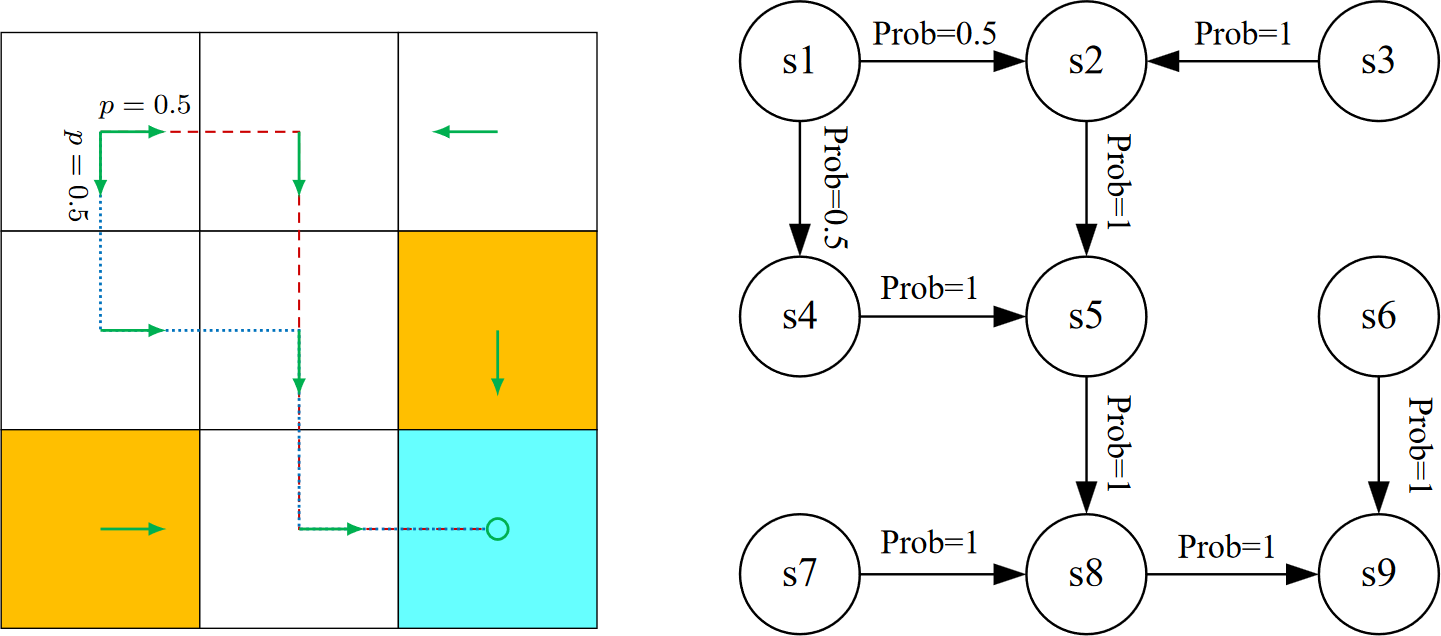
\includegraphics[width=.75\textwidth]{figures/ch3/3.mdp.png}
    \caption{The example grid as a Markov Process graph, where the nodes
    represent the states and the edges represent the state transitions.}
    \vspace{-10px}
    \caption*{\scriptsize{Source: \cite{zhao2024RLBook}}}
    \label{fig:mdp}
\end{figure}

\section{Causal Inference}

\cite{Neal_2020a}

\section{Generative Adversarial Networks}